\documentclass[twoside]{book}

% Packages required by doxygen
\usepackage{calc}
\usepackage{doxygen}
\usepackage{graphicx}
\usepackage[utf8]{inputenc}
\usepackage{makeidx}
\usepackage{multicol}
\usepackage{multirow}
\usepackage{textcomp}
\usepackage[table]{xcolor}

% Font selection
\usepackage[T1]{fontenc}
\usepackage{mathptmx}
\usepackage[scaled=.90]{helvet}
\usepackage{courier}
\usepackage{amssymb}
\usepackage{sectsty}
\renewcommand{\familydefault}{\sfdefault}
\allsectionsfont{%
  \fontseries{bc}\selectfont%
  \color{darkgray}%
}
\renewcommand{\DoxyLabelFont}{%
  \fontseries{bc}\selectfont%
  \color{darkgray}%
}

% Page & text layout
\usepackage{geometry}
\geometry{%
  a4paper,%
  top=2.5cm,%
  bottom=2.5cm,%
  left=2.5cm,%
  right=2.5cm%
}
\tolerance=750
\hfuzz=15pt
\hbadness=750
\setlength{\emergencystretch}{15pt}
\setlength{\parindent}{0cm}
\setlength{\parskip}{0.2cm}
\makeatletter
\renewcommand{\paragraph}{%
  \@startsection{paragraph}{4}{0ex}{-1.0ex}{1.0ex}{%
    \normalfont\normalsize\bfseries\SS@parafont%
  }%
}
\renewcommand{\subparagraph}{%
  \@startsection{subparagraph}{5}{0ex}{-1.0ex}{1.0ex}{%
    \normalfont\normalsize\bfseries\SS@subparafont%
  }%
}
\makeatother

% Headers & footers
\usepackage{fancyhdr}
\pagestyle{fancyplain}
\fancyhead[LE]{\fancyplain{}{\bfseries\thepage}}
\fancyhead[CE]{\fancyplain{}{}}
\fancyhead[RE]{\fancyplain{}{\bfseries\leftmark}}
\fancyhead[LO]{\fancyplain{}{\bfseries\rightmark}}
\fancyhead[CO]{\fancyplain{}{}}
\fancyhead[RO]{\fancyplain{}{\bfseries\thepage}}
\fancyfoot[LE]{\fancyplain{}{}}
\fancyfoot[CE]{\fancyplain{}{}}
\fancyfoot[RE]{\fancyplain{}{\bfseries\scriptsize Generated on Sat Feb 22 2014 15\-:33\-:56 for My Project by Doxygen }}
\fancyfoot[LO]{\fancyplain{}{\bfseries\scriptsize Generated on Sat Feb 22 2014 15\-:33\-:56 for My Project by Doxygen }}
\fancyfoot[CO]{\fancyplain{}{}}
\fancyfoot[RO]{\fancyplain{}{}}
\renewcommand{\footrulewidth}{0.4pt}
\renewcommand{\chaptermark}[1]{%
  \markboth{#1}{}%
}
\renewcommand{\sectionmark}[1]{%
  \markright{\thesection\ #1}%
}

% Indices & bibliography
\usepackage{natbib}
\usepackage[titles]{tocloft}
\setcounter{tocdepth}{3}
\setcounter{secnumdepth}{5}
\makeindex

% Hyperlinks (required, but should be loaded last)
\usepackage{ifpdf}
\ifpdf
  \usepackage[pdftex,pagebackref=true]{hyperref}
\else
  \usepackage[ps2pdf,pagebackref=true]{hyperref}
\fi
\hypersetup{%
  colorlinks=true,%
  linkcolor=blue,%
  citecolor=blue,%
  unicode%
}

% Custom commands
\newcommand{\clearemptydoublepage}{%
  \newpage{\pagestyle{empty}\cleardoublepage}%
}


%===== C O N T E N T S =====

\begin{document}

% Titlepage & ToC
\hypersetup{pageanchor=false}
\pagenumbering{roman}
\begin{titlepage}
\vspace*{7cm}
\begin{center}%
{\Large My Project }\\
\vspace*{1cm}
{\large Generated by Doxygen 1.8.6}\\
\vspace*{0.5cm}
{\small Sat Feb 22 2014 15:33:56}\\
\end{center}
\end{titlepage}
\clearemptydoublepage
\tableofcontents
\clearemptydoublepage
\pagenumbering{arabic}
\hypersetup{pageanchor=true}

%--- Begin generated contents ---
\chapter{Audio\-D\-X}
\label{md__r_e_a_d_m_e}
\hypertarget{md__r_e_a_d_m_e}{}
Audio Abstraction library for interfacing with hardware audio I/\-O devices

Currently only supports Windows.

Expanded A\-P\-I and Documentation coming soon...

Currently the A\-P\-I is N\-O\-T S\-T\-A\-B\-L\-E. The A\-P\-I W\-I\-L\-L C\-H\-A\-N\-G\-E as needed, solidifying at a later date. 
\chapter{Hierarchical Index}
\section{Class Hierarchy}
This inheritance list is sorted roughly, but not completely, alphabetically\-:\begin{DoxyCompactList}
\item \contentsline{section}{Audio\-D\-X\-:\-:Abstract\-Audio\-Device}{\pageref{class_audio_d_x_1_1_abstract_audio_device}}{}
\begin{DoxyCompactList}
\item \contentsline{section}{Audio\-D\-X\-:\-:Audio\-Capture\-Device}{\pageref{class_audio_d_x_1_1_audio_capture_device}}{}
\item \contentsline{section}{Audio\-D\-X\-:\-:Audio\-Playback\-Device}{\pageref{class_audio_d_x_1_1_audio_playback_device}}{}
\end{DoxyCompactList}
\item \contentsline{section}{Audio\-D\-X\-:\-:Abstract\-Audio\-Task}{\pageref{class_audio_d_x_1_1_abstract_audio_task}}{}
\begin{DoxyCompactList}
\item \contentsline{section}{Audio\-D\-X\-:\-:Audio\-Silence\-Task}{\pageref{class_audio_d_x_1_1_audio_silence_task}}{}
\end{DoxyCompactList}
\item \contentsline{section}{Audio\-D\-X\-:\-:Audio\-Buffer$<$ type, size $>$}{\pageref{struct_audio_d_x_1_1_audio_buffer}}{}
\item \contentsline{section}{Audio\-D\-X\-:\-:Audio\-Device\-Manager}{\pageref{class_audio_d_x_1_1_audio_device_manager}}{}
\item \contentsline{section}{Audio\-D\-X\-:\-:Audio\-Format}{\pageref{struct_audio_d_x_1_1_audio_format}}{}
\item \contentsline{section}{Taskable\-Callback}{\pageref{class_taskable_callback}}{}
\end{DoxyCompactList}

\chapter{Class Index}
\section{Class List}
Here are the classes, structs, unions and interfaces with brief descriptions\-:\begin{DoxyCompactList}
\item\contentsline{section}{\hyperlink{class_audio_d_x_1_1_abstract_audio_device}{Audio\-D\-X\-::\-Abstract\-Audio\-Device} }{\pageref{class_audio_d_x_1_1_abstract_audio_device}}{}
\item\contentsline{section}{\hyperlink{class_audio_d_x_1_1_abstract_audio_task}{Audio\-D\-X\-::\-Abstract\-Audio\-Task} }{\pageref{class_audio_d_x_1_1_abstract_audio_task}}{}
\item\contentsline{section}{\hyperlink{struct_audio_d_x_1_1_audio_buffer}{Audio\-D\-X\-::\-Audio\-Buffer$<$ type, size $>$} }{\pageref{struct_audio_d_x_1_1_audio_buffer}}{}
\item\contentsline{section}{\hyperlink{class_audio_d_x_1_1_audio_capture_device}{Audio\-D\-X\-::\-Audio\-Capture\-Device} }{\pageref{class_audio_d_x_1_1_audio_capture_device}}{}
\item\contentsline{section}{\hyperlink{class_audio_d_x_1_1_audio_device_manager}{Audio\-D\-X\-::\-Audio\-Device\-Manager} }{\pageref{class_audio_d_x_1_1_audio_device_manager}}{}
\item\contentsline{section}{\hyperlink{struct_audio_d_x_1_1_audio_format}{Audio\-D\-X\-::\-Audio\-Format} }{\pageref{struct_audio_d_x_1_1_audio_format}}{}
\item\contentsline{section}{\hyperlink{class_audio_d_x_1_1_audio_playback_device}{Audio\-D\-X\-::\-Audio\-Playback\-Device} }{\pageref{class_audio_d_x_1_1_audio_playback_device}}{}
\item\contentsline{section}{\hyperlink{class_audio_d_x_1_1_audio_silence_task}{Audio\-D\-X\-::\-Audio\-Silence\-Task} }{\pageref{class_audio_d_x_1_1_audio_silence_task}}{}
\item\contentsline{section}{\hyperlink{class_taskable_callback}{Taskable\-Callback} }{\pageref{class_taskable_callback}}{}
\end{DoxyCompactList}

\chapter{Class Documentation}
\hypertarget{class_audio_d_x_1_1_abstract_audio_device}{\section{Audio\-D\-X\-:\-:Abstract\-Audio\-Device Class Reference}
\label{class_audio_d_x_1_1_abstract_audio_device}\index{Audio\-D\-X\-::\-Abstract\-Audio\-Device@{Audio\-D\-X\-::\-Abstract\-Audio\-Device}}
}


\hyperlink{class_audio_d_x_1_1_abstract_audio_device}{Abstract\-Audio\-Device} is the base class for any system-\/recognized hardware.  




{\ttfamily \#include $<$Abstract\-Audio\-Device.\-h$>$}

Inheritance diagram for Audio\-D\-X\-:\-:Abstract\-Audio\-Device\-:\begin{figure}[H]
\begin{center}
\leavevmode
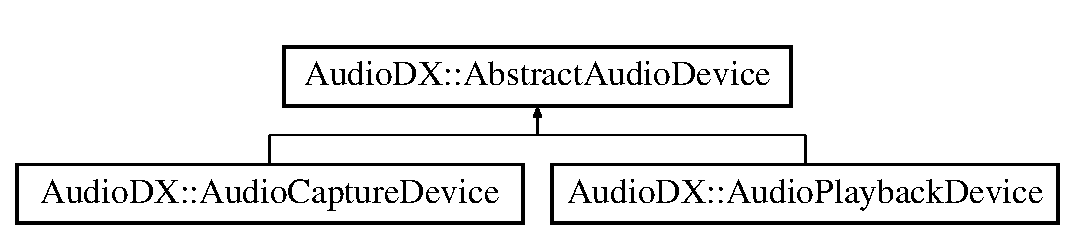
\includegraphics[height=2.000000cm]{class_audio_d_x_1_1_abstract_audio_device}
\end{center}
\end{figure}
\subsection*{Public Member Functions}
\begin{DoxyCompactItemize}
\item 
\hypertarget{class_audio_d_x_1_1_abstract_audio_device_a8bc151d485fbbea83d16e15abcc10df2}{virtual bool {\bfseries initialize} ()=0}\label{class_audio_d_x_1_1_abstract_audio_device_a8bc151d485fbbea83d16e15abcc10df2}

\item 
\hypertarget{class_audio_d_x_1_1_abstract_audio_device_a165b72ae32ab24d88018a2c4c7acd188}{virtual bool {\bfseries start} ()}\label{class_audio_d_x_1_1_abstract_audio_device_a165b72ae32ab24d88018a2c4c7acd188}

\item 
\hypertarget{class_audio_d_x_1_1_abstract_audio_device_aed3aa99e6eddb1ccb31e9c467afacc8e}{virtual bool {\bfseries stop} ()}\label{class_audio_d_x_1_1_abstract_audio_device_aed3aa99e6eddb1ccb31e9c467afacc8e}

\item 
\hypertarget{class_audio_d_x_1_1_abstract_audio_device_a5aa3d081130b952871e704d7ff005ec0}{virtual bool {\bfseries is\-Capture\-Device} () const }\label{class_audio_d_x_1_1_abstract_audio_device_a5aa3d081130b952871e704d7ff005ec0}

\item 
\hypertarget{class_audio_d_x_1_1_abstract_audio_device_a503b2a592b55b25903cc3f3e5389bd35}{virtual bool {\bfseries is\-Playback\-Device} () const }\label{class_audio_d_x_1_1_abstract_audio_device_a503b2a592b55b25903cc3f3e5389bd35}

\item 
\hypertarget{class_audio_d_x_1_1_abstract_audio_device_a35eddb40741fef8b011058cdef1c9daa}{virtual bool {\bfseries is\-Valid} () const }\label{class_audio_d_x_1_1_abstract_audio_device_a35eddb40741fef8b011058cdef1c9daa}

\item 
\hypertarget{class_audio_d_x_1_1_abstract_audio_device_a3910313a0578fa3c2b06501cc179af28}{virtual \hyperlink{struct_audio_d_x_1_1_audio_format}{Audio\-Format} {\bfseries get\-Audio\-Format} () const }\label{class_audio_d_x_1_1_abstract_audio_device_a3910313a0578fa3c2b06501cc179af28}

\item 
\hypertarget{class_audio_d_x_1_1_abstract_audio_device_a0c1724ac52fe657184986053994254f0}{virtual \hyperlink{class_audio_d_x_1_1_audio_buffer}{Audio\-Buffer} {\bfseries read\-From\-Buffer} ()=0}\label{class_audio_d_x_1_1_abstract_audio_device_a0c1724ac52fe657184986053994254f0}

\item 
\hypertarget{class_audio_d_x_1_1_abstract_audio_device_af7a91b536071e36806f1fc7eb029f872}{virtual bool {\bfseries write\-To\-Buffer} (const \hyperlink{class_audio_d_x_1_1_audio_buffer}{Audio\-Buffer} \&in, const \hyperlink{struct_audio_d_x_1_1_abstract_filter}{Abstract\-Filter} \&filter)=0}\label{class_audio_d_x_1_1_abstract_audio_device_af7a91b536071e36806f1fc7eb029f872}

\end{DoxyCompactItemize}
\subsection*{Protected Attributes}
\begin{DoxyCompactItemize}
\item 
\hypertarget{class_audio_d_x_1_1_abstract_audio_device_ae221dbe42940057a92ae0854f97d58d4}{std\-::shared\-\_\-ptr\\*
$<$ Abstract\-Audio\-Device\-Impl $>$ {\bfseries impl}}\label{class_audio_d_x_1_1_abstract_audio_device_ae221dbe42940057a92ae0854f97d58d4}

\end{DoxyCompactItemize}
\subsection*{Friends}
\begin{DoxyCompactItemize}
\item 
\hypertarget{class_audio_d_x_1_1_abstract_audio_device_aa3d09594a601dd4ef0a0bdd1c6ddd73c}{class {\bfseries Audio\-Device\-Manager}}\label{class_audio_d_x_1_1_abstract_audio_device_aa3d09594a601dd4ef0a0bdd1c6ddd73c}

\item 
\hypertarget{class_audio_d_x_1_1_abstract_audio_device_a04f96566766f09f439a3a13c5fcbe408}{class {\bfseries Audio\-Device\-Manager\-Impl}}\label{class_audio_d_x_1_1_abstract_audio_device_a04f96566766f09f439a3a13c5fcbe408}

\end{DoxyCompactItemize}


\subsection{Detailed Description}
\hyperlink{class_audio_d_x_1_1_abstract_audio_device}{Abstract\-Audio\-Device} is the base class for any system-\/recognized hardware. 

The documentation for this class was generated from the following files\-:\begin{DoxyCompactItemize}
\item 
Abstract\-Audio\-Device.\-h\item 
Abstract\-Audio\-Device.\-cpp\end{DoxyCompactItemize}

\hypertarget{class_audio_d_x_1_1_abstract_audio_task}{\section{Audio\-D\-X\-:\-:Abstract\-Audio\-Task Class Reference}
\label{class_audio_d_x_1_1_abstract_audio_task}\index{Audio\-D\-X\-::\-Abstract\-Audio\-Task@{Audio\-D\-X\-::\-Abstract\-Audio\-Task}}
}
Inheritance diagram for Audio\-D\-X\-:\-:Abstract\-Audio\-Task\-:\begin{figure}[H]
\begin{center}
\leavevmode
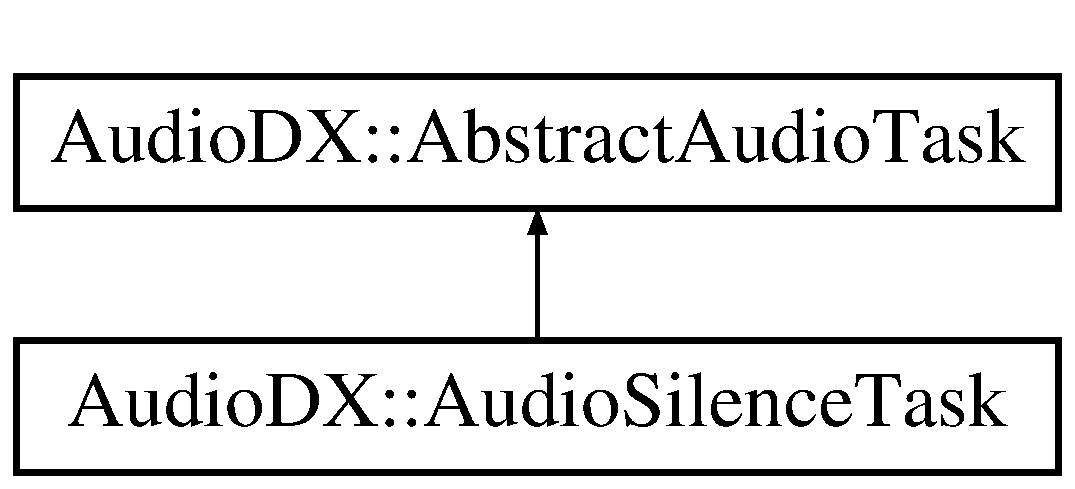
\includegraphics[height=2.000000cm]{class_audio_d_x_1_1_abstract_audio_task}
\end{center}
\end{figure}
\subsection*{Public Member Functions}
\begin{DoxyCompactItemize}
\item 
\hypertarget{class_audio_d_x_1_1_abstract_audio_task_adbb6d415b699251831bd119924ffcb32}{{\bfseries Abstract\-Audio\-Task} (\hyperlink{class_audio_d_x_1_1_abstract_audio_device}{Abstract\-Audio\-Device} $\ast$device)}\label{class_audio_d_x_1_1_abstract_audio_task_adbb6d415b699251831bd119924ffcb32}

\item 
\hypertarget{class_audio_d_x_1_1_abstract_audio_task_a1dabc891ee283d1e97c6cc3147fd79b8}{virtual void {\bfseries run} (\hyperlink{class_taskable_callback}{Taskable\-Callback} $\ast$callback=nullptr)=0}\label{class_audio_d_x_1_1_abstract_audio_task_a1dabc891ee283d1e97c6cc3147fd79b8}

\end{DoxyCompactItemize}
\subsection*{Protected Attributes}
\begin{DoxyCompactItemize}
\item 
\hypertarget{class_audio_d_x_1_1_abstract_audio_task_a5250f630cad2fc3501007f8e9712e847}{std\-::shared\-\_\-ptr\\*
$<$ \hyperlink{class_audio_d_x_1_1_abstract_audio_device}{Abstract\-Audio\-Device} $>$ {\bfseries m\-\_\-device}}\label{class_audio_d_x_1_1_abstract_audio_task_a5250f630cad2fc3501007f8e9712e847}

\end{DoxyCompactItemize}


The documentation for this class was generated from the following file\-:\begin{DoxyCompactItemize}
\item 
Tasks/Abstract\-Audio\-Task.\-h\end{DoxyCompactItemize}

\hypertarget{struct_audio_d_x_1_1_audio_buffer}{\section{Audio\-D\-X\-:\-:Audio\-Buffer$<$ type, size $>$ Struct Template Reference}
\label{struct_audio_d_x_1_1_audio_buffer}\index{Audio\-D\-X\-::\-Audio\-Buffer$<$ type, size $>$@{Audio\-D\-X\-::\-Audio\-Buffer$<$ type, size $>$}}
}


The documentation for this struct was generated from the following file\-:\begin{DoxyCompactItemize}
\item 
Audio\-Buffer.\-h\end{DoxyCompactItemize}

\hypertarget{class_audio_d_x_1_1_audio_capture_device}{\section{Audio\-D\-X\-:\-:Audio\-Capture\-Device Class Reference}
\label{class_audio_d_x_1_1_audio_capture_device}\index{Audio\-D\-X\-::\-Audio\-Capture\-Device@{Audio\-D\-X\-::\-Audio\-Capture\-Device}}
}
Inheritance diagram for Audio\-D\-X\-:\-:Audio\-Capture\-Device\-:\begin{figure}[H]
\begin{center}
\leavevmode
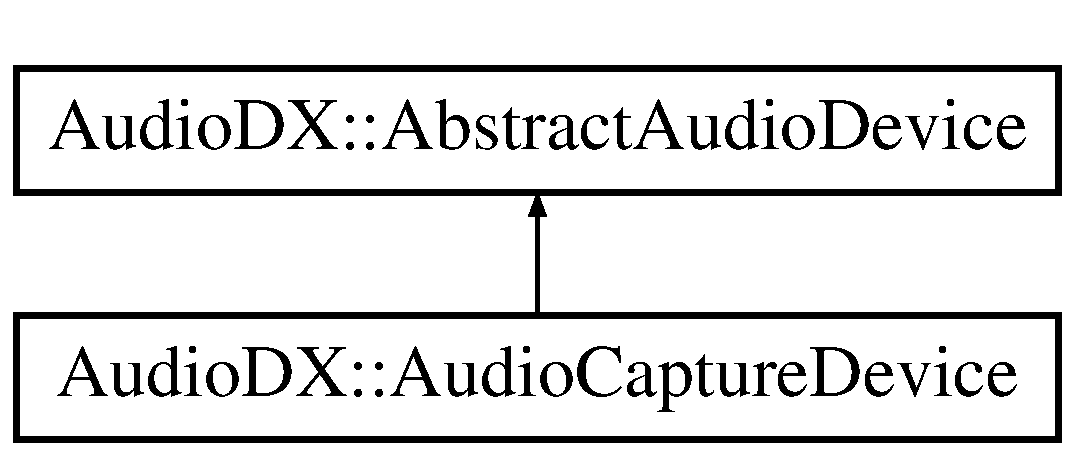
\includegraphics[height=2.000000cm]{class_audio_d_x_1_1_audio_capture_device}
\end{center}
\end{figure}
\subsection*{Public Member Functions}
\begin{DoxyCompactItemize}
\item 
\hypertarget{class_audio_d_x_1_1_audio_capture_device_ac250657c952e2d6b444f02437f1794e7}{virtual bool {\bfseries initialize} ()}\label{class_audio_d_x_1_1_audio_capture_device_ac250657c952e2d6b444f02437f1794e7}

\item 
\hypertarget{class_audio_d_x_1_1_audio_capture_device_af103510b605a3f09f45c9168a8314c2a}{virtual bool {\bfseries is\-Capture\-Device} () const }\label{class_audio_d_x_1_1_audio_capture_device_af103510b605a3f09f45c9168a8314c2a}

\end{DoxyCompactItemize}
\subsection*{Additional Inherited Members}


The documentation for this class was generated from the following files\-:\begin{DoxyCompactItemize}
\item 
Audio\-Capture\-Device.\-h\item 
Audio\-Capture\-Device.\-cpp\end{DoxyCompactItemize}

\hypertarget{class_audio_d_x_1_1_audio_device_manager}{\section{Audio\-D\-X\-:\-:Audio\-Device\-Manager Class Reference}
\label{class_audio_d_x_1_1_audio_device_manager}\index{Audio\-D\-X\-::\-Audio\-Device\-Manager@{Audio\-D\-X\-::\-Audio\-Device\-Manager}}
}
\subsection*{Public Member Functions}
\begin{DoxyCompactItemize}
\item 
\hypertarget{class_audio_d_x_1_1_audio_device_manager_abf9da36f8c05a6e21eb46a71e5370342}{bool {\bfseries initialize} ()}\label{class_audio_d_x_1_1_audio_device_manager_abf9da36f8c05a6e21eb46a71e5370342}

\item 
\hypertarget{class_audio_d_x_1_1_audio_device_manager_a16f6e3bad725b0cbcc412ad1d71c74fd}{bool {\bfseries un\-Initialize} ()}\label{class_audio_d_x_1_1_audio_device_manager_a16f6e3bad725b0cbcc412ad1d71c74fd}

\item 
\hypertarget{class_audio_d_x_1_1_audio_device_manager_ac28b6ccb55dd9298c87d3646551853f8}{std\-::vector$<$ std\-::shared\-\_\-ptr\\*
$<$ \hyperlink{class_audio_d_x_1_1_audio_playback_device}{Audio\-Playback\-Device} $>$ $>$ {\bfseries get\-Playback\-Devices} () const }\label{class_audio_d_x_1_1_audio_device_manager_ac28b6ccb55dd9298c87d3646551853f8}

\item 
\hypertarget{class_audio_d_x_1_1_audio_device_manager_a16ea9809c9a042ceeb0c29d39959862e}{std\-::vector$<$ std\-::shared\-\_\-ptr\\*
$<$ \hyperlink{class_audio_d_x_1_1_audio_capture_device}{Audio\-Capture\-Device} $>$ $>$ {\bfseries get\-Capture\-Devices} () const }\label{class_audio_d_x_1_1_audio_device_manager_a16ea9809c9a042ceeb0c29d39959862e}

\item 
\hypertarget{class_audio_d_x_1_1_audio_device_manager_a1cb22811ab6b73c1c0b4461870ec6f27}{std\-::vector$<$ std\-::shared\-\_\-ptr\\*
$<$ \hyperlink{class_audio_d_x_1_1_abstract_audio_device}{Abstract\-Audio\-Device} $>$ $>$ {\bfseries get\-All\-Devices} () const }\label{class_audio_d_x_1_1_audio_device_manager_a1cb22811ab6b73c1c0b4461870ec6f27}

\item 
\hypertarget{class_audio_d_x_1_1_audio_device_manager_aa9f75198d5d0b9442a31cf7006f3bab2}{bool {\bfseries is\-Initialized} () const }\label{class_audio_d_x_1_1_audio_device_manager_aa9f75198d5d0b9442a31cf7006f3bab2}

\end{DoxyCompactItemize}


The documentation for this class was generated from the following files\-:\begin{DoxyCompactItemize}
\item 
Audio\-Device\-Manager.\-h\item 
Audio\-Device\-Manager.\-cpp\end{DoxyCompactItemize}

\hypertarget{struct_audio_d_x_1_1_audio_format}{\section{Audio\-D\-X\-:\-:Audio\-Format Struct Reference}
\label{struct_audio_d_x_1_1_audio_format}\index{Audio\-D\-X\-::\-Audio\-Format@{Audio\-D\-X\-::\-Audio\-Format}}
}
\subsection*{Public Member Functions}
\begin{DoxyCompactItemize}
\item 
\hypertarget{struct_audio_d_x_1_1_audio_format_aae4df65348ca1230851036bb9fd91050}{bool {\bfseries operator==} (const \hyperlink{struct_audio_d_x_1_1_audio_format}{Audio\-Format} \&other) const }\label{struct_audio_d_x_1_1_audio_format_aae4df65348ca1230851036bb9fd91050}

\item 
\hypertarget{struct_audio_d_x_1_1_audio_format_a328ce800ed9717ce42c7bcab0fb176a2}{bool {\bfseries operator!=} (const \hyperlink{struct_audio_d_x_1_1_audio_format}{Audio\-Format} \&other) const }\label{struct_audio_d_x_1_1_audio_format_a328ce800ed9717ce42c7bcab0fb176a2}

\end{DoxyCompactItemize}
\subsection*{Public Attributes}
\begin{DoxyCompactItemize}
\item 
\hypertarget{struct_audio_d_x_1_1_audio_format_abb4ac7cdfaee71a384f897fb66dfbf6f}{unsigned int {\bfseries channels}}\label{struct_audio_d_x_1_1_audio_format_abb4ac7cdfaee71a384f897fb66dfbf6f}

\item 
\hypertarget{struct_audio_d_x_1_1_audio_format_abb6d613e6aa6fe3ea89346f928682ac2}{unsigned int {\bfseries samples\-Per\-Second}}\label{struct_audio_d_x_1_1_audio_format_abb6d613e6aa6fe3ea89346f928682ac2}

\item 
\hypertarget{struct_audio_d_x_1_1_audio_format_a1d3af66864e53a267e9b49b1689e7215}{unsigned int {\bfseries bits\-Per\-Block}}\label{struct_audio_d_x_1_1_audio_format_a1d3af66864e53a267e9b49b1689e7215}

\item 
\hypertarget{struct_audio_d_x_1_1_audio_format_a6fb2f886f394562d4b1c8d4f7986f59e}{unsigned int {\bfseries bits\-Per\-Sample}}\label{struct_audio_d_x_1_1_audio_format_a6fb2f886f394562d4b1c8d4f7986f59e}

\end{DoxyCompactItemize}


The documentation for this struct was generated from the following files\-:\begin{DoxyCompactItemize}
\item 
Audio\-Format.\-h\item 
Audio\-Format.\-cpp\end{DoxyCompactItemize}

\hypertarget{class_audio_d_x_1_1_audio_playback_device}{\section{Audio\-D\-X\-:\-:Audio\-Playback\-Device Class Reference}
\label{class_audio_d_x_1_1_audio_playback_device}\index{Audio\-D\-X\-::\-Audio\-Playback\-Device@{Audio\-D\-X\-::\-Audio\-Playback\-Device}}
}
Inheritance diagram for Audio\-D\-X\-:\-:Audio\-Playback\-Device\-:\begin{figure}[H]
\begin{center}
\leavevmode
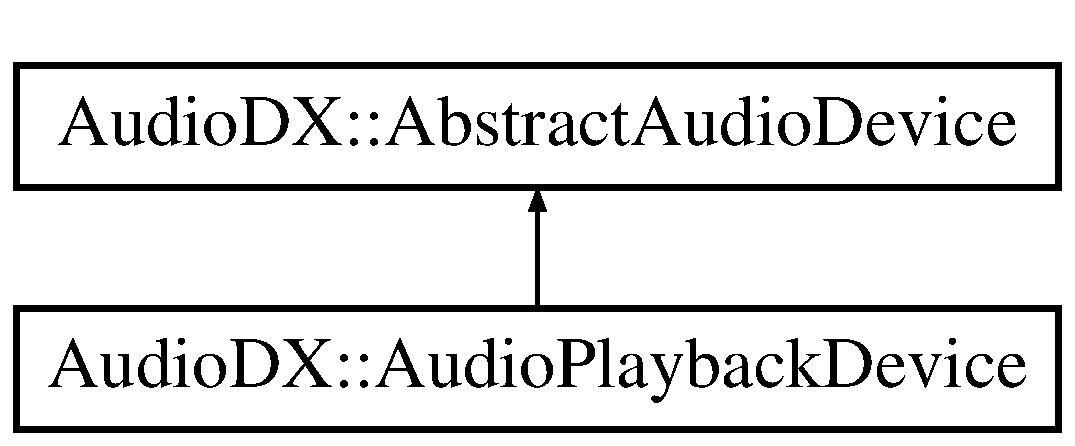
\includegraphics[height=2.000000cm]{class_audio_d_x_1_1_audio_playback_device}
\end{center}
\end{figure}
\subsection*{Public Member Functions}
\begin{DoxyCompactItemize}
\item 
\hypertarget{class_audio_d_x_1_1_audio_playback_device_abffabc4a3dbe82dfe059a8d5d8fd916c}{virtual bool {\bfseries initialize} ()}\label{class_audio_d_x_1_1_audio_playback_device_abffabc4a3dbe82dfe059a8d5d8fd916c}

\item 
\hypertarget{class_audio_d_x_1_1_audio_playback_device_ab3a966c43557f8cee9bac54d46ef08a0}{virtual bool {\bfseries is\-Playback\-Device} () const }\label{class_audio_d_x_1_1_audio_playback_device_ab3a966c43557f8cee9bac54d46ef08a0}

\item 
\hypertarget{class_audio_d_x_1_1_audio_playback_device_a2f018910e1511f29864ac8fb98b19e87}{virtual bool {\bfseries write\-To\-Buffer} (const \hyperlink{class_audio_d_x_1_1_audio_buffer}{Audio\-Buffer} \&in, const \hyperlink{struct_audio_d_x_1_1_abstract_filter}{Abstract\-Filter} \&filter=\hyperlink{struct_audio_d_x_1_1_abstract_filter}{Abstract\-Filter}())}\label{class_audio_d_x_1_1_audio_playback_device_a2f018910e1511f29864ac8fb98b19e87}

\item 
\hypertarget{class_audio_d_x_1_1_audio_playback_device_ae364b268314fbb1bea0bc25447b00088}{virtual \hyperlink{class_audio_d_x_1_1_audio_buffer}{Audio\-Buffer} {\bfseries read\-From\-Buffer} ()}\label{class_audio_d_x_1_1_audio_playback_device_ae364b268314fbb1bea0bc25447b00088}

\end{DoxyCompactItemize}
\subsection*{Additional Inherited Members}


The documentation for this class was generated from the following files\-:\begin{DoxyCompactItemize}
\item 
Audio\-Playback\-Device.\-h\item 
Audio\-Playback\-Device.\-cpp\end{DoxyCompactItemize}

\hypertarget{class_audio_d_x_1_1_audio_silence_task}{\section{Audio\-D\-X\-:\-:Audio\-Silence\-Task Class Reference}
\label{class_audio_d_x_1_1_audio_silence_task}\index{Audio\-D\-X\-::\-Audio\-Silence\-Task@{Audio\-D\-X\-::\-Audio\-Silence\-Task}}
}
Inheritance diagram for Audio\-D\-X\-:\-:Audio\-Silence\-Task\-:\begin{figure}[H]
\begin{center}
\leavevmode
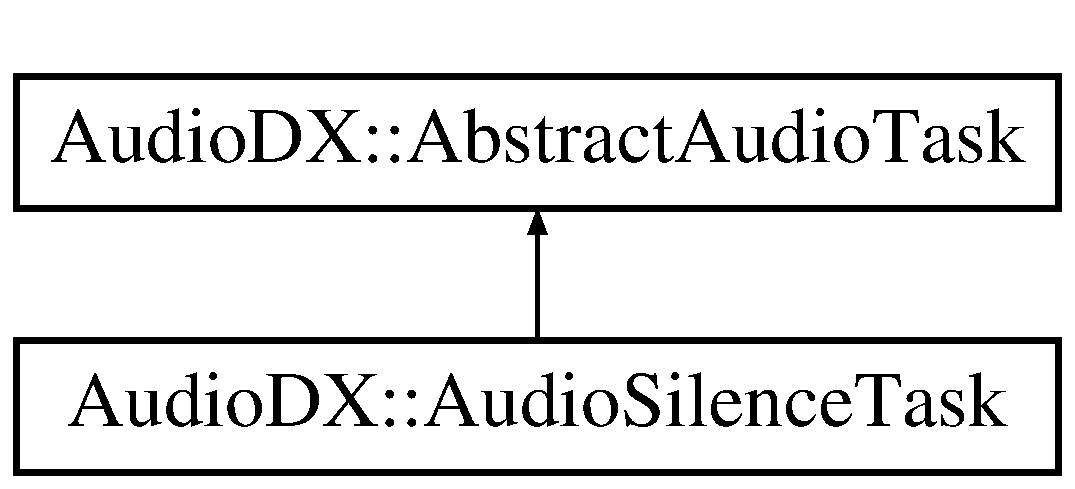
\includegraphics[height=2.000000cm]{class_audio_d_x_1_1_audio_silence_task}
\end{center}
\end{figure}
\subsection*{Public Member Functions}
\begin{DoxyCompactItemize}
\item 
\hypertarget{class_audio_d_x_1_1_audio_silence_task_a2365eef397d04ed2681a331b6d1baf3d}{void {\bfseries run} (\hyperlink{class_taskable_callback}{Taskable\-Callback} $\ast$callback=nullptr)}\label{class_audio_d_x_1_1_audio_silence_task_a2365eef397d04ed2681a331b6d1baf3d}

\end{DoxyCompactItemize}
\subsection*{Additional Inherited Members}


The documentation for this class was generated from the following files\-:\begin{DoxyCompactItemize}
\item 
Tasks/Audio\-Silence\-Task.\-h\item 
Tasks/Audio\-Silence\-Task.\-cpp\end{DoxyCompactItemize}

\hypertarget{class_taskable_callback}{\section{Taskable\-Callback Class Reference}
\label{class_taskable_callback}\index{Taskable\-Callback@{Taskable\-Callback}}
}
\subsection*{Public Member Functions}
\begin{DoxyCompactItemize}
\item 
\hypertarget{class_taskable_callback_ab97aa7fdd217837d1fac5fee72637b82}{virtual void {\bfseries update\-Progress} (unsigned int current, unsigned int total)}\label{class_taskable_callback_ab97aa7fdd217837d1fac5fee72637b82}

\item 
\hypertarget{class_taskable_callback_aa1382c7c0441664cac76a0861c2ba92b}{virtual void {\bfseries update\-Progress} (unsigned int current)}\label{class_taskable_callback_aa1382c7c0441664cac76a0861c2ba92b}

\item 
\hypertarget{class_taskable_callback_aa82a479049148db7abb3467df37de198}{virtual void {\bfseries stop\-Task} (bool stop=false)}\label{class_taskable_callback_aa82a479049148db7abb3467df37de198}

\end{DoxyCompactItemize}


The documentation for this class was generated from the following files\-:\begin{DoxyCompactItemize}
\item 
Utilities/Taskable\-Callback.\-h\item 
Utilities/Taskable\-Callback.\-cpp\end{DoxyCompactItemize}

%--- End generated contents ---

% Index
\newpage
\phantomsection
\addcontentsline{toc}{chapter}{Index}
\printindex

\end{document}
